\documentclass{article}

\title{Practice-2}
\author{2347139}
\date{\today}


\usepackage{listings}
\usepackage{color}
\usepackage{graphicx}

\definecolor{dkgreen}{rgb}{0,0.6,0}
\definecolor{gray}{rgb}{0.5,0.5,0.5}
\definecolor{mauve}{rgb}{0.58,0,0.82}

\lstset{frame=tb,
  language=Java,
  aboveskip=3mm,
  belowskip=3mm,
  showstringspaces=false,
  columns=flexible,
  basicstyle={\small\ttfamily},
  numbers=left,
  numberstyle=\tiny\color{gray},
  keywordstyle=\color{blue},
  commentstyle=\color{dkgreen},
  stringstyle=\color{mauve},
  breaklines=true,
  breakatwhitespace=true,
  tabsize=3
}
\begin{document}
\maketitle
\begin{lstlisting}
   // 4. Tell Me Why

public class Client1 {
    static void doCalc(byte... a) {
        System.out.print("byte...");
    }

    static void doCalc(long a, long b) {
        System.out.print("long, long");
    }

    static void doCalc(Byte s1, Byte s2) {
        System.out.print("Byte, Byte");
    }

    public static void main(String[] args) {
        byte b = 5;
        doCalc(b, b); // static methods placed within the same class can be called directlty, datatype
                      // is matched in the function call
    }
}

\end{lstlisting}

\section*{Output}
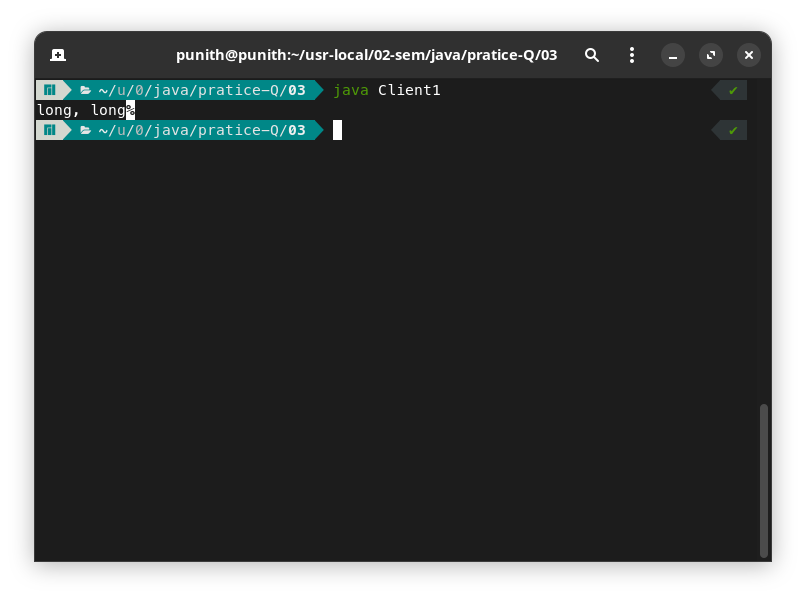
\includegraphics[width=11cm, height=9cm]{./images/01.png}
\begin{lstlisting}
    // 5.What gets printed on the standard output when the class below is compiled and executed. 

    public class ShortCkt {
        public static void main(String args[]) {
            int i = 0;
            boolean t = true;
            boolean f = false, b;
            b = (t | ((i++) == 0));
            b = (f | ((i += 2) > 0));
            System.out.println(i);
        }
    }    
 \end{lstlisting}
 \section*{Output}
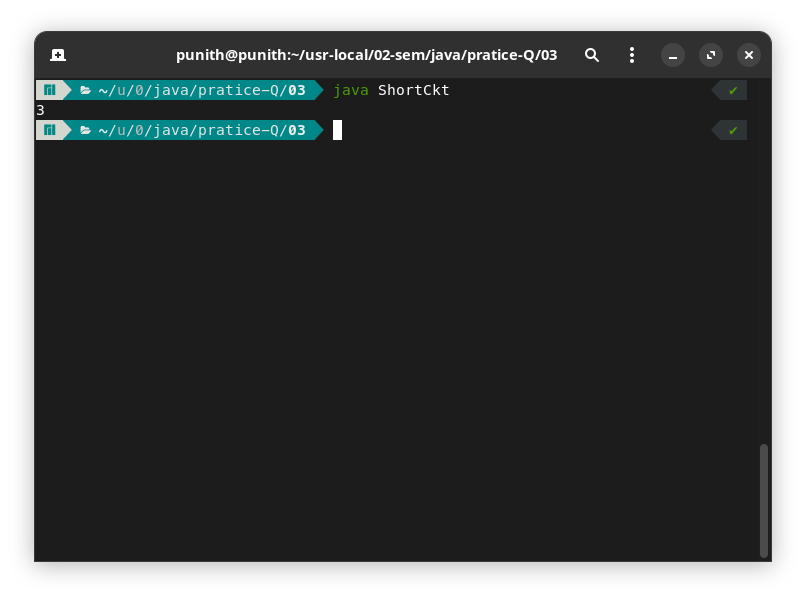
\includegraphics[width=11cm, height=9cm]{./images/02.png}


 \begin{lstlisting}
    //6.  What gets displayed on the screen when the following program is compiled and run. 

public class test {
    public static void main(String args[]) {
        boolean x = true;
        int a;
        if (x)
            a = x ? 1 : 2;
        else
            a = x ? 3 : 4;
        System.out.println(a);
    }
}

 \end{lstlisting}

 \section*{Output}
 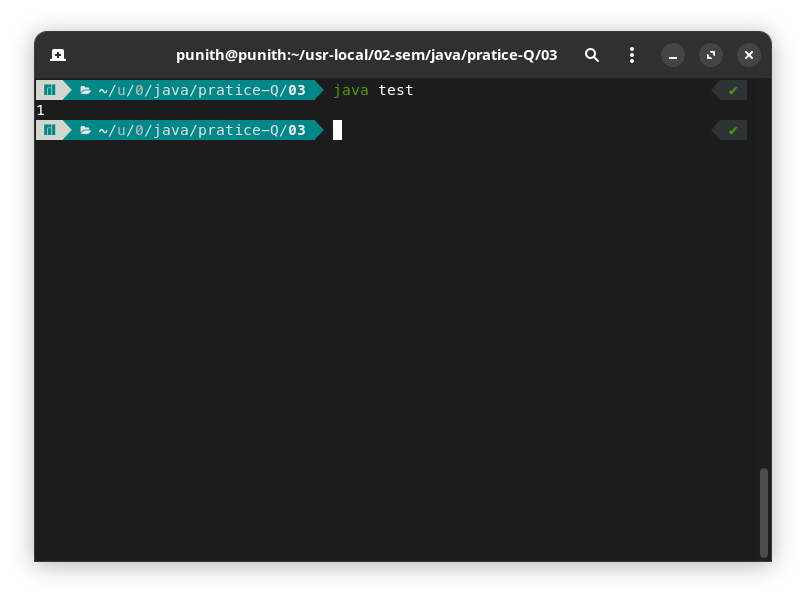
\includegraphics[width=11cm, height=9cm]{./images/03.png}


 \begin{lstlisting}
    // What is the result when this code is executed?

    class One {
        public One() {
            System.out.print(1);
        }
    }
    
    class Two extends One {
        public Two() {
            System.out.print(2);
        }
    }
    
    class Three extends Two {
        public Three() {
            System.out.print(3);
        }
    }
    
    public class Numbers {
        public static void main(String[] argv) {
            new Three();
        }
    }
       
 \end{lstlisting}

 \section*{Output}
 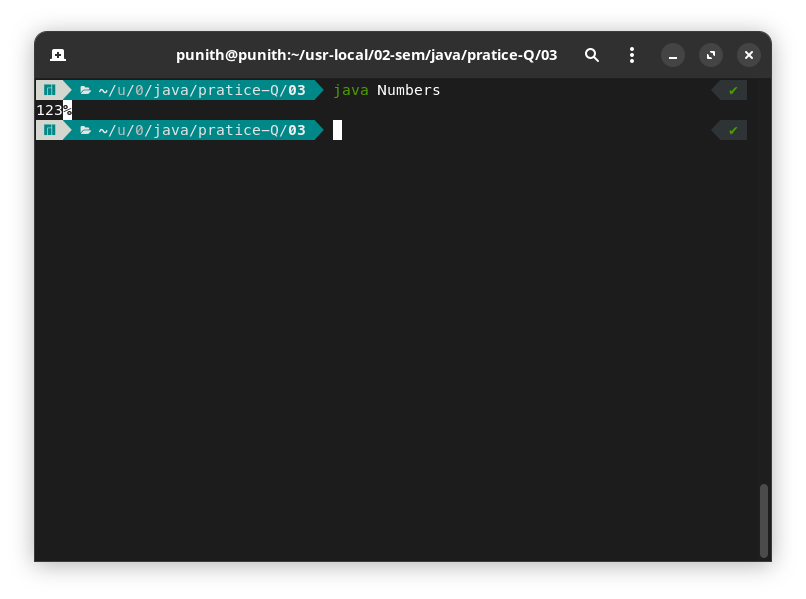
\includegraphics[width=11cm, height=9cm]{./images/04.png}


 \begin{lstlisting}
    // public What all gets printed when the following program is compiled and run. 

    public class test1 {
        public static void main(String args[]) {
            int i = 0, j = 2;
            do {
                i = ++i;
                j--;
            } while (j > 0);
            System.out.println(i);
        }
    }
 \end{lstlisting}
 \section*{Output}
 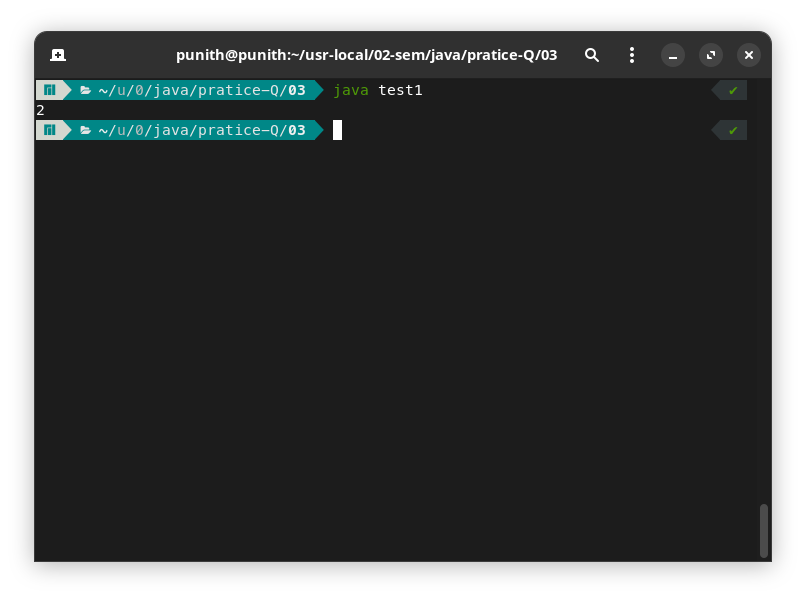
\includegraphics[width=11cm, height=9cm]{./images/05.png}
 \begin{lstlisting}
    // What is the result?

    class test3 {
        public static void checkSomething(String str) {
            int check = 4;
            if (check == str.length()) {
                System.out.print(str.charAt(check -= 1) + ", ");
            } else {
                System.out.print(str.charAt(0) + ", ");
            }
        }
    
        public static void makinStrings() {
            String s = "Fred";
            s = s + "47";
            s = s.substring(2, 5);
            s = s.toUpperCase();
            System.out.println(s.toString());
            // return s.toString();
        }
    
        public static void main(String args[]) {
            checkSomething("four");
            checkSomething("tee");
            checkSomething("to");
    
            // 11Q
            makinStrings();
    
        }
    }
    
    // 21.test("four");
    // 22.test("tee");
    // test("to");
    
 \end{lstlisting}
 \section*{Output}
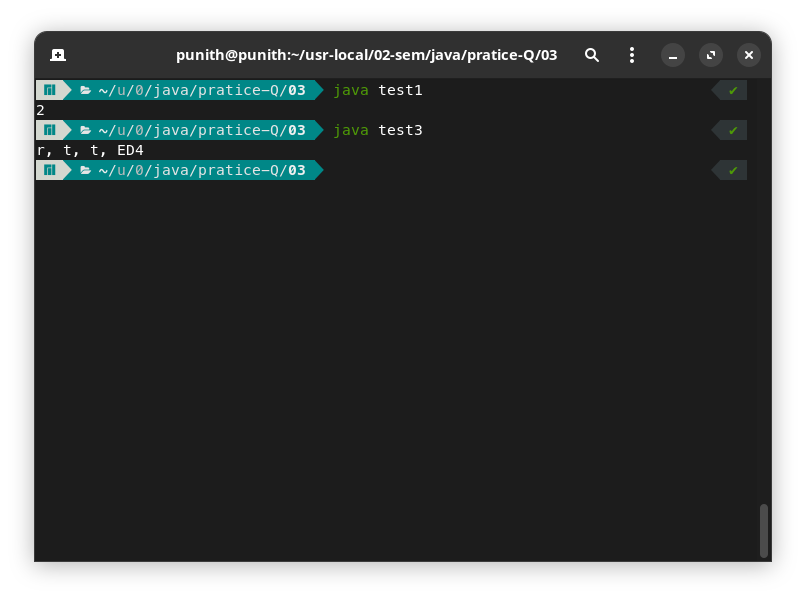
\includegraphics[width=11cm, height=9cm]{./images/06.png}
 \begin{lstlisting}
    public class Main {
        static void increment(int index) {
            index++;
        }
    
        public static void main(String[] args) {
            int i = 0;
            increment(i);
            i++;
            System.out.println(i);
        }
    
    }
    
 \end{lstlisting}
 \section*{Output}
 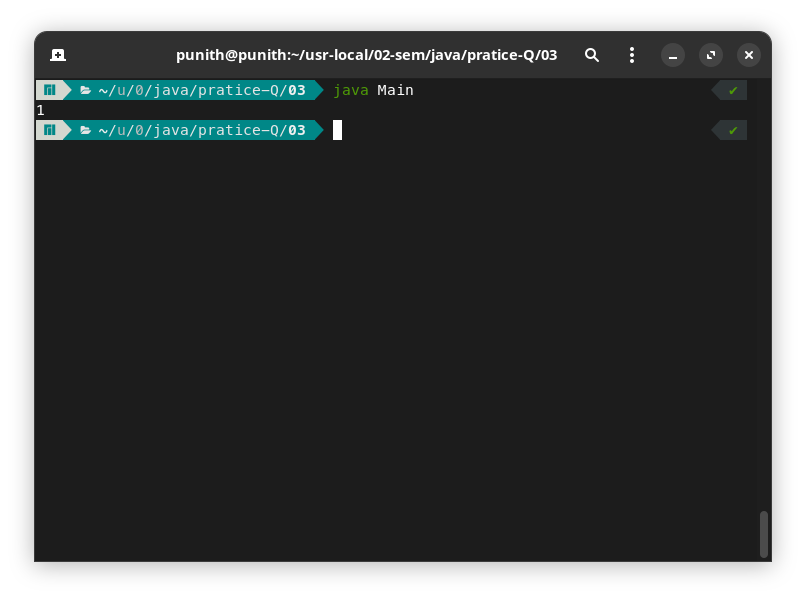
\includegraphics[width=11cm, height=9cm]{./images/07.png}
 \begin{lstlisting}
    public class Last {
        public static void main(String[] args) {
            Integer i = new Integer(1) + new Integer(2);
            switch (i) {
                case 3:
                    System.out.println("three");
                    break;
                default:
                    System.out.println("other");
                    break;
            }
        }
    }
    
 \end{lstlisting}
 \section*{Output}
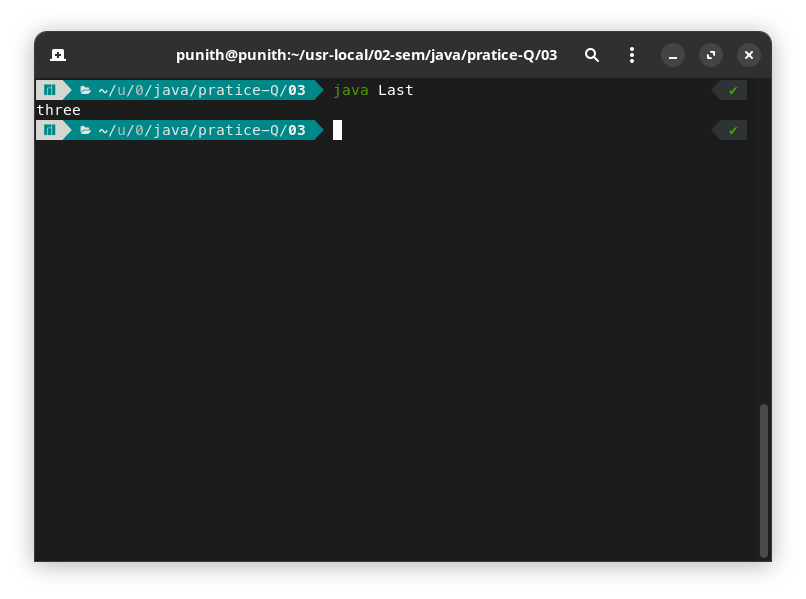
\includegraphics[width=11cm, height=9cm]{./images/08.png}

\end{document}
